\documentclass{beamer}
\mode<presentation>
\usepackage{amsmath}
\usepackage{amssymb}
%\usepackage{advdate}
\usepackage{adjustbox}
\usepackage{subcaption}
\usepackage{enumitem}
\usepackage{multicol}
\usepackage{mathtools}
\usepackage{listings}
\usepackage{float}
\usepackage{graphicx}
\usepackage{url}
\def\UrlBreaks{\do\/\do-}
\usetheme{Boadilla}
\usecolortheme{lily}
\setbeamertemplate{footline}
{
  \leavevmode%
  \hbox{%
  \begin{beamercolorbox}[wd=\paperwidth,ht=2.25ex,dp=1ex,right]{author in head/foot}%
    \insertframenumber{} / \inserttotalframenumber\hspace*{2ex} 
  \end{beamercolorbox}}%
  \vskip0pt%
}
\setbeamertemplate{navigation symbols}{}

\providecommand{\nCr}[2]{\,^{#1}C_{#2}} % nCr
\providecommand{\nPr}[2]{\,^{#1}P_{#2}} % nPr
\providecommand{\mbf}{\mathbf}
\providecommand{\pr}[1]{\ensuremath{\Pr\left(#1\right)}}
\providecommand{\qfunc}[1]{\ensuremath{Q\left(#1\right)}}
\providecommand{\sbrak}[1]{\ensuremath{{}\left[#1\right]}}
\providecommand{\lsbrak}[1]{\ensuremath{{}\left[#1\right.}}
\providecommand{\rsbrak}[1]{\ensuremath{{}\left.#1\right]}}
\providecommand{\brak}[1]{\ensuremath{\left(#1\right)}}
\providecommand{\lbrak}[1]{\ensuremath{\left(#1\right.}}
\providecommand{\rbrak}[1]{\ensuremath{\left.#1\right)}}
\providecommand{\cbrak}[1]{\ensuremath{\left\{#1\right\}}}
\providecommand{\lcbrak}[1]{\ensuremath{\left\{#1\right.}}
\providecommand{\rcbrak}[1]{\ensuremath{\left.#1\right\}}}
\theoremstyle{remark}
\newtheorem{rem}{Remark}
\newcommand{\sgn}{\mathop{\mathrm{sgn}}}
\providecommand{\abs}[1]{\left\vert#1\right\vert}
\providecommand{\res}[1]{\Res\displaylimits_{#1}} 
\providecommand{\norm}[1]{\lVert#1\rVert}
\providecommand{\mtx}[1]{\mathbf{#1}}
\providecommand{\mean}[1]{E\left[ #1 \right]}
\providecommand{\fourier}{\overset{\mathcal{F}}{ \rightleftharpoons}}
%\providecommand{\hilbert}{\overset{\mathcal{H}}{ \rightleftharpoons}}
\providecommand{\system}{\overset{\mathcal{H}}{ \longleftrightarrow}}
	%\newcommand{\solution}[2]{\textbf{Solution:}{#1}}
%\newcommand{\solution}{\noindent \textbf{Solution: }}
\providecommand{\dec}[2]{\ensuremath{\overset{#1}{\underset{#2}{\gtrless}}}}
\newcommand{\myvec}[1]{\ensuremath{\begin{pmatrix}#1\end{pmatrix}}}
\let\vec\mathbf

\lstset{
language=C,
frame=single, 
breaklines=true,
columns=fullflexible
}

\numberwithin{equation}{section}

\title{Presentation - Matgeo}
\author{Aryansingh Sonaye \\
AI25BTECH11032 \\
EE1030 - Matrix Theory}

\date{\today} 
\begin{document}

\begin{frame}
\titlepage
\end{frame}

\section{Problem}
\begin{frame}
\frametitle{Problem Statement}
\textbf{Problem 4.8.28}

Find the equation of the plane passing through the intersection of the planes
\begin{align}
\vec{r}\cdot(\hat{\imath}+\hat{\jmath}+\hat{k}) &= 1, \\[4pt]
\vec{r}\cdot(2\hat{\imath}+3\hat{\jmath}-\hat{k}) + 4 &= 0,
\end{align}
which is parallel to the $X$--axis. Hence, find the distance of the plane from the $X$--axis.
\end{frame}

\section{Solution}
\subsection{Description of Variables used}
\begin{frame}
\frametitle{Description of Variables used}
\begin{table}[H]
\centering
\begin{tabular}{|c |c|}
\hline
Quantity & Value \\
\hline
Normal of $\Pi_1$ & $\vec{n}_1=\myvec{1\\1\\1}$ \\
\hline
Right-hand side of $\Pi_1$ & $b_1=1$ \\
\hline
Normal of $\Pi_2$ & $\vec{n}_2=\myvec{2\\3\\-1}$ \\
\hline
Right-hand side of $\Pi_2$ & $b_2=-4$ \\
\hline
$X$--axis direction & $\vec{e}_1=\myvec{1\\0\\0}$ \\
\hline
\end{tabular}
\caption{Input values for the problem}
\end{table}


\end{frame}

\subsection{Theoretical Solution }
\begin{frame}
\frametitle{Theoretical Solution}
We first find the line of intersection of the given planes.  
Stacking the two plane equations in matrix form gives
\begin{align}
\vec{A}\vec{r} &= \vec{b}, \\
\vec{A} &= \myvec{\vec{n}_1^\top \\[4pt] \vec{n}_2^\top}
= \myvec{1 & 1 & 1 \\[4pt] 2 & 3 & -1}, \\
\vec{b} &= \myvec{1\\[4pt]-4}.
\end{align}

The augmented matrix is reduced as follows:
\begin{align}
\myvec{1 & 1 & 1 & |&1 \\[4pt] 2 & 3 & -1 & |&-4}
&\xrightarrow{R_2\leftarrow R_2-2R_1}
\myvec{1 & 1 & 1 & |&1 \\[4pt] 0 & 1 & -3 & |&-6} \\[8pt]
&\xrightarrow{R_1\leftarrow R_1-R_2}
\myvec{1 & 0 & 4 & |&7 \\[4pt] 0 & 1 & -3 & |&-6}.
\end{align}

\end{frame}

\begin{frame}
\frametitle{Theoretical Solution}
Thus the line of intersection can be expressed as
\begin{align}
\vec{r} &= \vec{r}_p + t\,\vec{d}, \\
\vec{r}_p &= \myvec{7\\[4pt]-6\\[4pt]0}, \\
\vec{d} &= \myvec{-4\\[4pt]3\\[4pt]1}.
\end{align}

Next, since the required plane is parallel to the $X$--axis, its normal $\vec{n}$ must be orthogonal to $\vec{e}_1$.  
Also, since the plane contains the intersection line, $\vec{n}$ must be orthogonal to $\vec{d}$.  
Hence the system is
\begin{align}
\vec{e}_1^\top \vec{n} &= 0, \\
\vec{d}^\top \vec{n} &= 0.
\end{align}

\end{frame}

\begin{frame}
\frametitle{Theoretical Solution}
Writing this in matrix form:
\begin{align}
\myvec{\vec{e}_1^\top \\[4pt] \vec{d}^\top}\vec{n}
&= \myvec{1 & 0 & 0 \\[4pt]-4 & 3 & 1}\vec{n}
= \myvec{0\\0}.
\end{align}

The augmented matrix reduces as
\begin{align}
\myvec{1 & 0 & 0 & |&0 \\[4pt]-4 & 3 & 1 & |&0}
&\xrightarrow{R_2\leftarrow R_2+4R_1}
\myvec{1 & 0 & 0 & |&0 \\[4pt]0 & 3 & 1 & |&0}.
\end{align}

From this we conclude
\begin{align}
n_x &= 0, \\
3n_y + n_z &= 0.
\end{align}
\end{frame}

\begin{frame}
\frametitle{Theoretical Solution}
Choosing a convenient scale, we may take
\begin{align}
\vec{n} &= \myvec{0\\[4pt]-1\\[4pt]3}.
\end{align}

Now the constant term of the plane is obtained by substituting a point $\vec{r}_p$ on the line:
\begin{align}
c &= \vec{n}^\top \vec{r}_p, \\
c &= \myvec{0 & -1 & 3}\myvec{7\\[4pt]-6\\[4pt]0}, \\
c &= 6.
\end{align}

Therefore, the equation of the required plane is
\begin{align}
\vec{n}^\top\vec{r} - c &= 0, \\
\vec{n}^\top\vec{r} - 6 &= 0.
\end{align}


\end{frame}

\begin{frame}
\frametitle{Theoretical Solution}
Finally, the distance of this plane from the $X$--axis is
\begin{align}
d &= \frac{|c|}{\|\vec{n}\|}, \\
d &= \frac{6}{\sqrt{\vec{n}^\top\vec{n}}}, \\
d &= \frac{6}{\sqrt{10}}.
\end{align}

\textbf{Final Answer}

\begin{align}
\boxed{\;\vec{n}^\top\vec{r} - c = 0\;}, \qquad
\boxed{\;\vec{n} = \myvec{0\\[4pt]-1\\[4pt]3}, \; c = 6\;}, \qquad
\boxed{\;\mathrm{distance} = \tfrac{6}{\sqrt{10}}\; }.
\end{align}


\end{frame}







\subsection{Plot}
\begin{frame}
    \frametitle{Plot}
\begin{figure}[H]
   \centering
   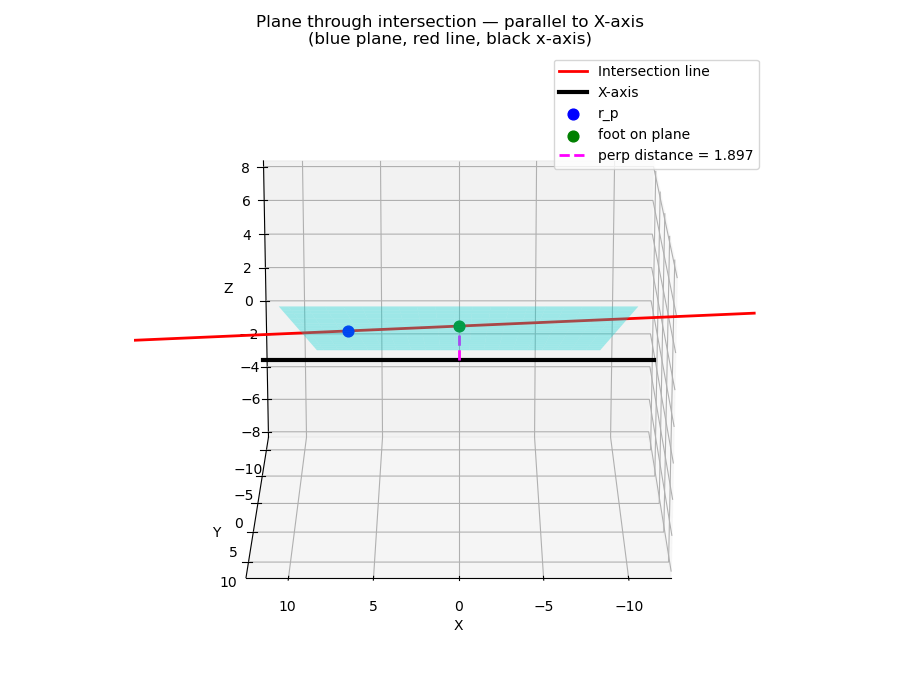
\includegraphics[width=0.9\columnwidth]{figs/new_plane.png}
   \caption{}
   \label{}
   \end{figure}
\end{frame}

\begin{frame}[fragile]
    \frametitle{Code - C}
    \begin{lstlisting}
#include <math.h>

#define EPS 1e-9

// Row reduction to Reduced Row Echelon Form (RREF)
void row_reduce(int rows, int cols, double *M) {
    int r = 0; // pivot row
    for (int c = 0; c < cols - 1 && r < rows; c++) {
        // 1. Find pivot
        int pivot = r;
        for (int i = r+1; i < rows; i++) {
            if (fabs(M[i*cols + c]) > fabs(M[pivot*cols + c])) {
                pivot = i;
            }
        }
        if (fabs(M[pivot*cols + c]) < EPS) continue;


    \end{lstlisting}
    \end{frame}

    \begin{frame}[fragile]
    \frametitle{Code - C}
    \begin{lstlisting}

        // 2. Swap rows if needed
        if (pivot != r) {
            for (int j = 0; j < cols; j++) {
                double tmp = M[r*cols + j];
                M[r*cols + j] = M[pivot*cols + j];
                M[pivot*cols + j] = tmp;
            }
        }

        // 3. Normalize pivot row
        double div = M[r*cols + c];
        for (int j = c; j < cols; j++) {
            M[r*cols + j] /= div;
        }



\end{lstlisting}
\end{frame}

    \begin{frame}[fragile]
    \frametitle{Code - C}
    \begin{lstlisting}
    
        // 4. Eliminate in all other rows
        for (int i = 0; i < rows; i++) {
            if (i == r) continue;
            double factor = M[i*cols + c];
            for (int j = c; j < cols; j++) {
                M[i*cols + j] -= factor * M[r*cols + j];
            }
        }
        r++;
    }
}






\end{lstlisting}
\end{frame}

\begin{frame}[fragile]
    \frametitle{Code - Python(with shared C code)}
    The code to obtain the required plot is
    \begin{lstlisting}
import ctypes
import numpy as np
import matplotlib.pyplot as plt

# Load C shared library
lib = ctypes.CDLL("./librowreduce.so")
lib.row_reduce.argtypes = (ctypes.c_int, ctypes.c_int,
                           ctypes.POINTER(ctypes.c_double))
lib.row_reduce.restype = None

\end{lstlisting}
\end{frame}
\begin{frame}[fragile]
\frametitle{Code - Python(with shared C code)}
\begin{lstlisting}
def row_reduce_numpy(A):
    """Run row_reduce from C on numpy array A (augmented matrix)."""
    rows, cols = A.shape
    A_flat = (ctypes.c_double * (rows*cols))(*A.flatten())
    lib.row_reduce(rows, cols, A_flat)
    return np.array(A_flat).reshape(rows, cols)

    
# Problem setup
n1 = np.array([1,1,1], dtype=float)
b1 = 1.0
n2 = np.array([2,3,-1], dtype=float)
b2 = -4.0
e1 = np.array([1,0,0], dtype=float)

\end{lstlisting}
\end{frame}

\begin{frame}[fragile]
\frametitle{Code - Python(with shared C code)}
\begin{lstlisting}
# Step 1: Line of intersection
M_line = np.array([[*n1, b1],
                   [*n2, b2]], dtype=float)
R_line = row_reduce_numpy(M_line)

# Particular point rp and direction d
rp = np.array([R_line[0,3], R_line[1,3], 0])   # set z=0 for particular solution
d  = np.array([-R_line[0,2], -R_line[1,2], 1]) # free variable = z

print("Particular point r_p =", rp)
print("Direction d =", d)

# Step 2: Normal vector
M_normal = np.array([[*e1, 0],
                     [*d,  0]], dtype=float)
R_normal = row_reduce_numpy(M_normal)
\end{lstlisting}
\end{frame}

\begin{frame}[fragile]
\frametitle{Code - Python(with shared C code)}
\begin{lstlisting}
# Extract n: last variable free = 1
n = np.array([-R_normal[0,2], -R_normal[1,2], 1])
c = np.dot(n, rp)

print("Normal vector n =", n)
print("Plane constant c =", c)

# Step 3: Distance from x-axis
p = np.array([0.0,0.0,0.0])  # any point on x-axis
dist = abs(np.dot(n,p) - c) / np.linalg.norm(n)
print("Distance from x-axis =", dist)

# Step 4: Plot figure
fig = plt.figure(figsize=(8,6))
ax = fig.add_subplot(111, projection='3d')

# Line of intersection


\end{lstlisting}
\end{frame}

\begin{frame}[fragile]
\frametitle{Code - Python(with shared C code)}
\begin{lstlisting}
t_vals = np.linspace(-5, 5, 100)
line_pts = np.array([rp + t*d for t in t_vals])
ax.plot(line_pts[:,0], line_pts[:,1], line_pts[:,2],
        color="red", lw=2, label="Line of intersection")

# Plane surface (n = [0,-1,1] , solve for Y in terms of X,Z)
x_vals = np.linspace(-5, 10, 30)
z_vals = np.linspace(-6, 6, 30)
X, Z = np.meshgrid(x_vals, z_vals)
Y = (c - n[0]*X - n[2]*Z)/n[1]
ax.plot_surface(X, Y, Z, alpha=0.5, color="blue")

# X-axis
ax.plot([-10, 10], [0, 0], [0, 0], 'k-', lw=3, label="X-axis")


\end{lstlisting}
\end{frame}

\begin{frame}[fragile]
\frametitle{Code - Python(with shared C code)}
\begin{lstlisting}
# Formatting
ax.set_xlabel("X")
ax.set_ylabel("Y")
ax.set_zlabel("Z")
ax.set_xlim(-10, 10)
ax.set_ylim(-10, 10)
ax.set_zlim(-6, 6)
ax.view_init(elev=20, azim=45)  # adjust angle to see parallelism
ax.legend()
plt.savefig("plane.png")
plt.show()

\end{lstlisting}
\end{frame}


\begin{frame}[fragile]
\frametitle{Code - Python only}
\begin{lstlisting}
import numpy as np
import matplotlib.pyplot as plt

# Gauss-Jordan row reduction with partial pivoting (returns RREF)
# A is a numpy array (rows x cols), operates on a copy
def row_reduce(A_in, eps=1e-12):
    A = A_in.astype(float).copy()
    rows, cols = A.shape
    r = 0
    for c in range(cols - 1):  # last column is RHS
        if r >= rows:
            break

        # partial pivot: find row with max abs in column c at or below r
        pivot = r
        maxv = abs(A[pivot, c])

\end{lstlisting}
\end{frame}
\begin{frame}[fragile]
\frametitle{Code - Python only}
\begin{lstlisting}
        for i in range(r+1, rows):
            v = abs(A[i, c])
            if v > maxv:
                maxv = v
                pivot = i
        if maxv < eps:
            # no pivot in this column
            continue
        # swap if needed
        if pivot != r:
            A[[r, pivot], :] = A[[pivot, r], :]
        # normalize pivot row
        div = A[r, c]
        A[r, c:] = A[r, c:] / div
        # eliminate in all other rows

\end{lstlisting}
\end{frame}

\begin{frame}[fragile]
\frametitle{Code - Python only}
\begin{lstlisting}
        for i in range(rows):
            if i == r:
                continue
            factor = A[i, c]
            if abs(factor) > eps:
                A[i, c:] = A[i, c:] - factor * A[r, c:]
        r += 1
    # zero-out tiny values for neatness
    A[np.abs(A) < 1e-12] = 0.0
    return A

# Problem data
n1 = np.array([1.0, 1.0, 1.0])
b1 = 1.0
n2 = np.array([2.0, 3.0, -1.0])
b2 = -4.0
e1 = np.array([1.0, 0.0, 0.0])  # x-axis direction

\end{lstlisting}
\end{frame}

\begin{frame}[fragile]
\frametitle{Code - Python only}
\begin{lstlisting}
# Step 1: line of intersection [A|b]
M_line = np.vstack([np.hstack([n1, b1]), np.hstack([n2, b2])])
R_line = row_reduce(M_line)
print("RREF (line system):\n", R_line)

# Interpret RREF: assume last variable (z) free -> set z = t
# Row form: row0: x + a z = r0  => x = r0 - a t
#           row1: y + b z = r1  => y = r1 - b t
rp = np.array([R_line[0,3], R_line[1,3], 0.0])      # t=0
d  = np.array([-R_line[0,2], -R_line[1,2], 1.0])   # coefficients of t
print("\nParticular point r_p =", rp)
print("Direction d =", d)
\end{lstlisting}
\end{frame}

\begin{frame}[fragile]
\frametitle{Code - Python only}
\begin{lstlisting}
# Step 2: plane normal: solve [e1^T; d^T] n = 0
M_norm = np.vstack([np.hstack([e1, 0.0]), np.hstack([d, 0.0])])
R_norm = row_reduce(M_norm)
print("\nRREF (normal system):\n", R_norm)

# choose last variable free = 1 -> n = [-R[0,2], -R[1,2], 1]
n = np.array([-R_norm[0,2], -R_norm[1,2], 1.0])
# scale normal to an integer-like/clean vector for nicer printing (optional)
# avoid scaling if zero
if np.linalg.norm(n) > 1e-12:
    # scale to make components integers if possible (here we know integers)
    # but we won't force scale; keep as computed
    pass
\end{lstlisting}
\end{frame}

\begin{frame}[fragile]
\frametitle{Code - Python only}
\begin{lstlisting}
c = float(np.dot(n, rp))
print("\nNormal n =", n)
print("Plane constant c =", c)

# Step 3: distance from x-axis
# Choose a convenient point on x-axis p0 = (0,0,0)
# distance = | n.p0 - c | / ||n|| = | -c | / ||n||
# Also compute the perpendicular foot point from p0 onto plane:
# foot = p0 + ((c - n.p0)/||n||^2) * n
p0 = np.array([0.0, 0.0, 0.0])
n_norm = np.linalg.norm(n)
if n_norm < 1e-12:
    dist = float('nan')
    foot = None
else:
    dist = abs(np.dot(n, p0) - c) / n_norm
    foot = p0 + ((c - np.dot(n, p0)) / (n_norm**2)) * n

\end{lstlisting}
\end{frame}

\begin{frame}[fragile]
\frametitle{Code - Python only}
\begin{lstlisting}
print("\nDistance from x-axis =", dist)
print("Perpendicular foot on plane from origin (x-axis point) =", foot)

# Step 4: Plot everything clearly showing plane parallel to x-axis
fig = plt.figure(figsize=(9,7))
ax = fig.add_subplot(111, projection='3d')

# plot line of intersection (parametric)
t_vals = np.linspace(-6, 6, 201)
line_pts = np.array([rp + t*d for t in t_vals])
ax.plot(line_pts[:,0], line_pts[:,1], line_pts[:,2], color='red', lw=2, label='Intersection line')
\end{lstlisting}
\end{frame}

\begin{frame}[fragile]
\frametitle{Code - Python only}
\begin{lstlisting}
# Create plane grid such that plane visibly looks parallel to x-axis:
if abs(n[1]) > 1e-9:
    # make grid in X and Z (X free direction shows parallelism)
    x_vals = np.linspace(-10, 10, 40)
    z_vals = np.linspace(-8, 8, 40)
    X, Z = np.meshgrid(x_vals, z_vals)
    Y = (c - n[0]*X - n[2]*Z) / n[1]
    ax.plot_surface(X, Y, Z, alpha=0.35, color='cyan', rstride=2, cstride=2, linewidth=0)
else:
    # if n[1] ~ 0, solve for X instead (rare)
    y_vals = np.linspace(-10, 10, 40)
    z_vals = np.linspace(-8, 8, 40)
    Y, Z = np.meshgrid(y_vals, z_vals)
    X = (c - n[1]*Y - n[2]*Z) / n[0]
    ax.plot_surface(X, Y, Z, alpha=0.35, color='cyan', rstride=2, cstride=2, linewidth=0)
\end{lstlisting}
\end{frame}

\begin{frame}[fragile]
\frametitle{Code - Python only}
\begin{lstlisting}
# plot x-axis bold
ax.plot([-12, 12], [0,0], [0,0], color='k', lw=3, label='X-axis')

# mark particular point rp and foot
ax.scatter([rp[0]],[rp[1]],[rp[2]], color='blue', s=60, label='r_p')
if foot is not None:
    ax.scatter([foot[0]],[foot[1]],[foot[2]], color='green', s=60, label='foot on plane')
    # draw perpendicular segment from p0 on x-axis to foot
    ax.plot([p0[0], foot[0]], [p0[1], foot[1]], [p0[2], foot[2]],
            color='magenta', lw=2, linestyle='--', label=f'perp distance = {dist:.3f}')

# labels and view - choose view that shows parallelism (look along x to show plane side)
\end{lstlisting}
\end{frame}

\begin{frame}[fragile]
\frametitle{Code - Python only}
\begin{lstlisting}
ax.set_xlabel('X')
ax.set_ylabel('Y')
ax.set_zlabel('Z')
ax.set_xlim(-12, 12)
ax.set_ylim(-12, 12)
ax.set_zlim(-8, 8)

# set viewing angle so x-axis appears lateral to plane: azim  90 looks down +x direction
ax.view_init(elev=18, azim=90)
ax.legend()
ax.set_title("Plane through intersection - parallel to X-axis\n(blue plane, red line, black x-axis)")
plt.tight_layout()
plt.savefig("new_plane.png")
plt.show()
\end{lstlisting}
\end{frame}

\end{document}
